%
% $Id: AttributeSet.java 15 2010-10-11 16:16:32Z justinkamerman $ 
%
% $LastChangedDate: 2010-10-11 13:16:32 -0300 (Mon, 11 Oct 2010) $ 
% 
% $LastChangedBy: justinkamerman $
%

\documentclass[10pt]{report}
\usepackage{graphicx}
\usepackage{amsmath}
\usepackage{setspace}			
\onehalfspacing

\title{CS6735 Programming Assignment 2}
\author{Justin Kamerman 3335272}
\date{\today}

\begin{document}
\maketitle
% No chapter numbers
\renewcommand*\thesection{\arabic{section}}

%----------------------------------------
% Assignment
%----------------------------------------
\section{Assignment}
\begin{enumerate} 
\item Implement Na\"{\i}ve Bayes using Java. Evaluate your implementation
  on the datasets in data.zip using 10 times 5-fold cross-validation,
  and report the average accuracy and standard deviation. All datasets
  are for UCI machine learning repository. You can check the detailed
  descriptions from the following link: 
 
http://www.ics.uci.edu/~mlearn/MLRepository.html

For breast cancer data see:
http://archive.ics.uci.edu/ml/datasets/Breast+Cancer+Wisconsin+%28Diagnostic%29

For car data see:
http://archive.ics.uci.edu/ml/datasets/Car+Evaluation

For ecoli data see:http://archive.ics.uci.edu/ml/datasets/Ecoli

For letter recognition data see:
http://archive.ics.uci.edu/ml/datasets/Letter+Recognition

For mushroom data see: http://archive.ics.uci.edu/ml/datasets/Mushroom

\item Bonus question: For a given data set, can we detect whether the
  conditional independent assumption is true or not? How? Can we
  observe that naïve Bayes works well only on the data sets on which
  the conditional independent assumption is true or roughly true? You
  may need to check some reference papers. 
\end{enumerate}

%----------------------------------------
% Learning Algorithm
%----------------------------------------
\section{Learning Algorithm}
\label{sec:learningalgorithm}

A Java program was written implementing the Na\"{i}ve Bayes Classifier as
described in ~\cite{Mitchell1997}. During the learning phase of the
algorithm, the program calculates a marginal probability vector, with
each position in the vector corresponding to a possible target
value. A three-dimensional conditional probability matrix is
populated, one dimesion corresponding to target value, another
dimension corresponding to attribute class, and a third dimension
corresponding to attribute value domain. In estimating conditional
probabilites, the \textbf{m-estimate} technique described in
~\cite{Mitchell1997} is used:

\begin{equation*}
P(A_{j}=a_{k}|C=c_{i}) = \frac{n_{c} + mp}{n + m}
\end{equation*}

where, for a particular training set, n is the cardinality of the
subset for which classification \(c_h\) holds and \(n_c\), the
cardinality of the subset of instances for which classification
\(c_i\) holds and attribute class \(A_j\) has value \(a_k\). \(p\) is
a prior estimate of the probability we wish to calculate. In this
case, we assume uniform distribution i.e. if the attribute in question
has \(k\) possible values, we assign \(p = \frac{1}{k}\). \(m\) is a
constant value which we call the \textit{equivalent sample size} and
determines how heavily to weight p relative to the observed
data. 

Using \textit{m-estimate} to estimate conditional probabilites
addresses the problem of a sparse probability matrix. Without
\textit{m-estimate}, matrix nodes which are not represented in the
training data are set to zero, resulting in a biased underestimation
of probabilities calculated uisng these terms. Using
\textit{m-estimate}, matrix nodes not represented in the training data
are set to \(\frac{mp}{n + m}\) instead.

Missing attribute values are handled by preprocessing data sets,
replacing missing attribute value with the most probable value for the
attribute in the data set.

\cite{*}

%----------------------------------------
% Data Sets
%----------------------------------------
\section{Data Sets}
Program expects data in CSV format with attributes occurring first and
classification at the end of each line. All data files have been
preprocessed to fit this format.


\subsection*{car.data}
\begin{itemize}
\item Number of Instances: 1728
\item Number of Attributes: 6
\item Attribute Values:
  \\\\
  \begin{left}
    \begin{tabular}{ l l }
      buying     & v-high, high, med, low \\
      maint      & v-high, high, med, low \\
      doors      & 2, 3, 4, 5-more \\
      persons    & 2, 4, more \\
      lug\_boot  & small, med, big \\
      safety     & low, med, high \\
    \end{tabular}
  \end{left}
  \\
\item Missing Attribute Values: none
\item Class Distribution (number of instances per class)
  \\\\
  \begin{left}
    \begin{tabular}{ l l }
      unacc   &  1210 \\
      acc     &   384 \\   
      good    &    69 \\     
      v-good  &    65 \\
    \end{tabular}
  \end{left}
\end{itemize}


\subsection*{ecoli.data}
\begin{itemize}
\item Number of Instances:  336
\item Number of Attributes: 7 
\item Attribute Values:
  \\\\
  \begin{left}
    \begin{tabular}{ l p{10cm} }
      mcg  &   McGeoch's method for signal sequence recognition. \\
      gvh  &   von Heijne's method for signal sequence recognition. \\
      lip  &   von Heijne's Signal Peptidase II consensus sequence score. Binary attribute. \\
      chg  &   Presence of charge on N-terminus of predicted lipoproteins. Binary attribute. \\
      aac  &   score of discriminant analysis of the amino acid content of outer membrane and periplasmic proteins. \\
      alm1 &   score of the ALOM membrane spanning region prediction program. \\
      alm2 &   score of ALOM program after excluding putative cleavable signal regions from the sequence. \\
    \end{tabular}
  \end{left}
  \\   
\item Missing Attribute Values: none.
\item Class Distribution (number of instances per class)
  \\\\
  \begin{left}
    \begin{tabular}{ l l }
      cp    &      143 \\
      im    &       77 \\               
      pp    &       52 \\
      imU   &       35 \\
      om    &       20 \\
      omL   &        5 \\
      imL   &        2 \\
      imS   &        2 \\
    \end{tabular}
  \end{left}
\end{itemize}


\subsection*{mushroom.data}
\begin{itemize}
\item Number of Instances: 8124
\item Number of Attributes: 22
\item Attribute Information:
  \\\\
  \begin{left}
    \begin{tabular}{ l p{10cm} }
      cap-shape                 &     bell=b, conical=c, convex=x, flat=f, knobbed=k, sunken=s \\
      cap-surface               &     fibrous=f, grooves=g, scaly=y, smooth=s \\
      cap-color                 &     brown=n, buff=b, cinnamon=c, gray=g, green=r, pink=p, purple=u, red=e, white=w, yellow=y \\
      bruises?                  &     bruises=t, no=f \\
      odor                      &     almond=a, anise=l, creosote=c, fishy=y, foul=f, musty=m, none=n, pungent=p, spicy=s \\
      gill-attachment           &     attached=a, descending=d, free=f, notched=n \\
      gill-spacing              &     close=c, crowded=w, distant=d \\
      gill-size                 &     broad=b, narrow=n \\
      gill-color                &     black=k, brown=n, buff=b, chocolate=h, gray=g, green=r, orange=o, pink=p, purple=u, red=e, white=w, yellow=y \\
      stalk-shape               &     enlarging=e, tapering=t \\
      stalk-root                &     bulbous=b, club=c, cup=u, equal=e, rhizomorphs=z, rooted=r, missing=? \\
      stalk-surface-above-ring  &     fibrous=f, scaly=y, silky=k, smooth=s \\
      stalk-surface-below-ring  &     fibrous=f, scaly=y, silky=k, smooth=s \\
      stalk-color-above-ring    &     brown=n, buff=b, cinnamon=c, gray=g, orange=o, pink=p, red=e, white=w, yellow=y \\
      stalk-color-below-ring    &     brown=n, buff=b, cinnamon=c, gray=g, orange=o, pink=p, red=e, white=w, yellow=y \\
      veil-type                 &     partial=p, universal=u \\
      veil-color                &     brown=n, orange=o, white=w, yellow=y \\
      ring-number               &     none=n, one=o, two=t \\
      ring-type                 &     cobwebby=c, evanescent=e, flaring=f, large=l, none=n, pendant=p, sheathing=s, zone=z \\
      spore-print-color         &     black=k, brown=n, buff=b, chocolate=h, green=r, orange=o, purple=u, white=w, yellow=y \\
      population                &     abundant=a, clustered=c, numerous=n, scattered=s, several=v, solitary=y \\
      habitat                   &     grasses=g, leaves=l, meadows=m, paths=p, urban=u, waste=w, woods=d \\
    \end{tabular}
  \end{left}

\item Missing Attribute Values: 2480, all for attribute #11.
\item Class Distribution: 
  \\\\
  \begin{left}
    \begin{tabular}{ l l }
      edible:     &  4208 (51.8\%) \\
      poisonous:  &  3916 (48.2\%) \\
      total:      &  8124 instances \\
    \end{tabular}
  \end{left}
\end{itemize}


\subsection*{letter-recognition.data}
\begin{itemize}
\item Number of Instances: 20000
\item Number of Attributes: 17 (Letter category and 16 numeric features)
\item Attribute Information:
  \\\\
  \begin{left}
    \begin{tabular}{ l p{10cm} }
      lettr	   &    capital letter	(26 values from A to Z) \\
      x-box	   &    horizontal position of box	(integer) \\
      y-box	   &    vertical position of box	(integer) \\
      width	   &    width of box			(integer) \\
      high 	   &    height of box			(integer) \\
      onpix	   &    total # on pixels		(integer) \\
      x-bar	   &    mean x of on pixels in box	(integer) \\
      y-bar	   &    mean y of on pixels in box	(integer) \\
      x2bar	   &    mean x variance			(integer) \\
      y2bar	   &    mean y variance			(integer) \\
      xybar	   &    mean x y correlation		(integer) \\
      x2ybr	   &    mean of x * x * y		(integer) \\
      xy2br	   &    mean of x * y * y		(integer) \\
      x-ege	   &    mean edge count left to right	(integer) \\
      xegvy	   &    correlation of x-ege with y	(integer) \\
      y-ege	   &    mean edge count bottom to top	(integer) \\
      yegvx	   &    correlation of y-ege with x	(integer) \\
    \end{tabular}
  \end{left}

\item Missing Attribute Values: None
\item Class Distribution:
  \\\\
  \begin{left}
    \begin{tabular}{ l l l l l l l }
 	789 A	   & 766 B     & 736 C     & 805 D	 & 768 E	   & 775 F     & 773 G \\
 	734 H	   & 755 I     & 747 J     & 739 K	 & 761 L	   & 792 M     & 783 N \\
 	753 O	   & 803 P     & 783 Q     & 758 R	 & 748 S	   & 796 T     & 813 U \\
 	764 V	   & 752 W     & 787 X     & 786 Y	 & 734 Z \\
    \end{tabular}
  \end{left}
\end{itemize}


\subsection*{breast-cancer.data}
\begin{itemize}
\item Number of Instances: 699
\item Number of Attributes: 10
\item Attribute Information: (class attribute has been moved to last column)
  \\\\
  \begin{left}
    \begin{tabular}{ l l }
      Clump Thickness               &  1 - 10  \\
      Uniformity of Cell Size       &  1 - 10  \\
      Uniformity of Cell Shape      &  1 - 10  \\
      Marginal Adhesion             &  1 - 10  \\
      Single Epithelial Cell Size   &  1 - 10  \\
      Bare Nuclei                   &  1 - 10  \\
      Bland Chromatin               &  1 - 10  \\
      Normal Nucleoli               &  1 - 10  \\
      Mitoses                       &  1 - 10  \\
    \end{tabular}
  \end{left}

\item Missing attribute values: 16
\item Class distribution: (2 for benign, 4 for malignant)
  \\\\
  \begin{left}
    \begin{tabular}{ l l }
      Benign       &  458 (65.5\%) \\
      Malignant    &  241 (34.5\%) \\
    \end{tabular}
  \end{left}
\end{itemize}


%----------------------------------------
% Program Design
%----------------------------------------
\section{Program Design}
The Na\"{\i}ve algorithms are implemented by a Java program. The only
external dependency is on the Apache commons-cli library for parsing
commend line options. To that end, the program is operated from the
command line, taking options listed in table
~\ref{tab:commandline}. Wrapper scripts, \textit{run.sh} and
\textit{run.bat} are provided as a convenience for executing the
program on UNIX and Windows platforms respectively. The header
comments in each script contain the command lines used for executing
the program with the varous data files provided.
\\
\begin{table}[h]
  \centering
  \begin{tabular}{ |l|p{10cm}|} 
    \hline
    Option & Description \\ \hline
    -f \<arg\>  &  Path of data file \\ \hline
    -i \<arg\>  &  Number of iterations to perform. Default is 10 \\ \hline
    -n \<arg\>  &  A comma-separated list of attribute names, matching
    the order in which they appear in the data file \\ \hline
    -o \<arg\>  &  Number of folds to create in the training data
    during. Default is 5. \\ \hline
    -m \<arg\>  &  m-estimate equivalent sample size \\ \hline
    -h          &  Print help message \\ \hline
  \end{tabular}
  \caption{Command line options}
  \label{tab:commandline}
\end{table}
\\\\
The program parses a data file, assumed to contain a set of training
instances on each line. Each training instance line is a
comma-separated list of attribute values terminated by a
classification or target value. Of the training data supplied for the
assignment, some had to be preprocessed to fit the expected format.

The program then executes a number of iterations (default is 10) over
the entire data set. During each iteration, the data set is folded
(default is 5 times), the training set used to create a Na\"\{i}ve
  Bayes Classifier. The instances in the test set are then evaluated 
  by the classifier and the accuracy of the classifications is
  recorded for each test set evaluated. After the final iteration is
  complete, the mean accuracy and standard deviation are calculated
  and output by the program.

The program implements various mechanism to facilitate
debugging. Throughout the code, log statements have been added using
the Java logging framework. The logging output is controlled for
individual classes via the \textit{logging.properties} file which the program
read on startup.

\begin{figure}
  \begin{center}
	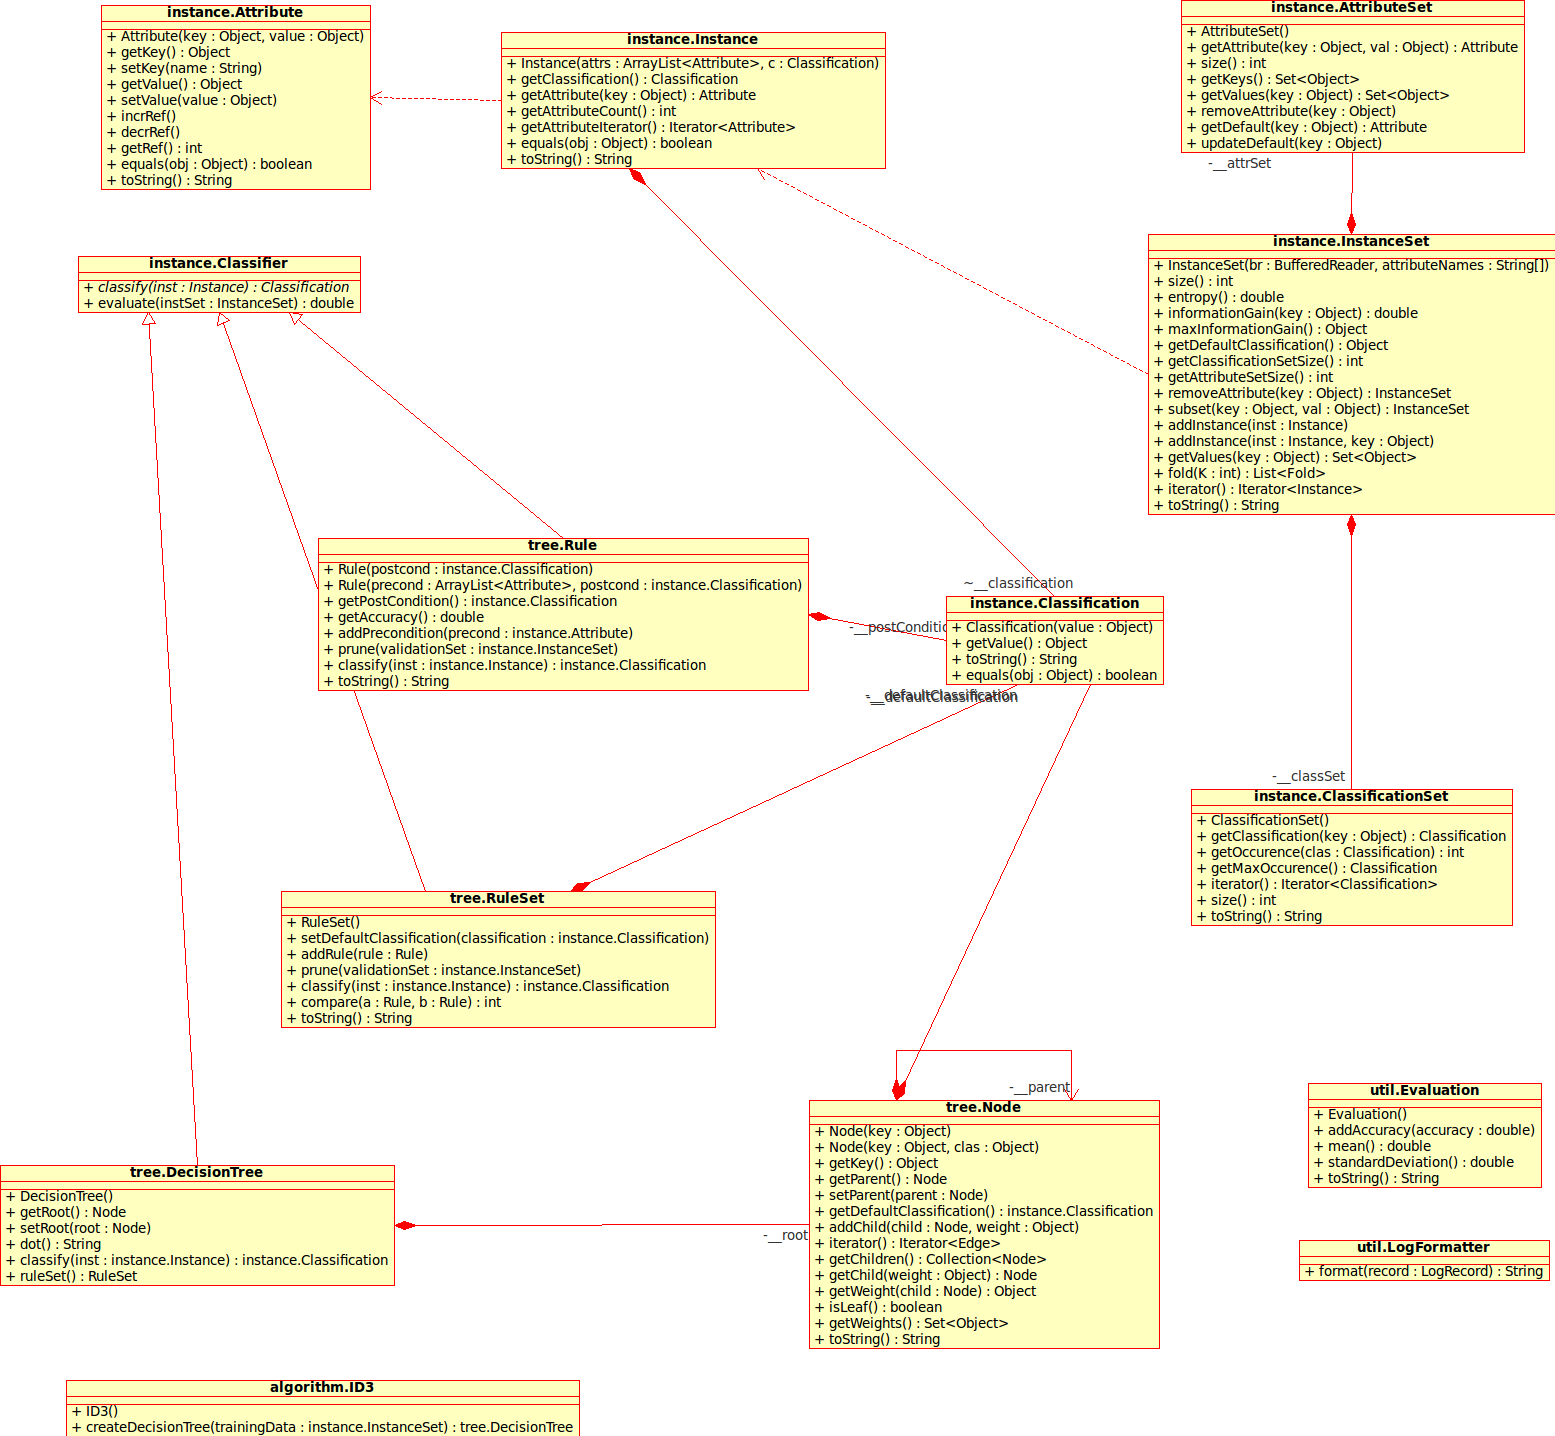
\includegraphics[width=\textwidth,height=!]{uml}
  \end{center}
  \caption{UML class diagram}
  \label{fig:uml}
\end{figure} 

The implementation classes and their relationships are represented in a UML
class diagram in Figure \ref{fig:uml}. Following is a brief
description of each class:

\begin{itemize}
\item \textbf{Attribute} represents an attribute's name and value.

\item \textbf{AttributeSet} is a collection of attributes. It has
  convenience functions to determine attribute value range and
  probabilities of discrete values.

\item \textbf{Classification} represents an instance's classification
  or the value of the target function.

\item \textbf{ClassificationSet} is a collection of
  classifications. It has convenience functions to determine
  classification value range and probabilities of each
  classification. These functions are used extensively during the
  entropy calculation. 

\item \textbf{Classifier} is an interface implemented by any class
  which can take an instance and generate a classification for that
  instance. The interface is implemented by the \textit{DecisionTree},
  \textit{Rule}, and \textit{RuleSet} classes.

\item \textbf{Evaluation} is a helper class for capturing test run
  accuracies and calculating final mean and standard deviation values.

\item \textbf{Fold} is an encapsulation of a training and a test set.

\item \textbf{Instance} represents a collection of attributes and
  their classification. In the case of training data, we use the
  classification to select the target hypothesis. In the case of test
  data, the classification is used to validate output of the target
  hypothesis.

\item \textbf{InstanceSet} is a collection of \textit{Instances}. This is the
  class that parses the data file and generates individual
  Instances. Functions exist to calculate entropy and information
  gain, create a subset of instance based on a particular attribute's
  value and fold the set of instances to create test and training sets
  of instances.

\item \textbf{LogFormatter} is a helper class to format log messages.

\item \textbf{Main} is the class which is started from the command
  line. It parses command line options and starts the test iterations.

\item \textbf{NaiveBayes} creates a Na\"{\i}ve Bayes classifier
  given a training data \textit{InstanceSet}. It calculates marginal
  and conditional probabilites and populates a probability matrix
  within the \textit{NaiveBayesClassifier}. It uses the m-estimation
  technique to estimate conditional probabilities.

\item \textbf{NaiveBayesClassifier} classifies an \textit{Instance}
  using the Na\"{i}ve Bayes Classifier algorithm, based on a matrix of
  marginal and conditional probabilities which are calculated from a
  previously seen training set.

\end{itemize}


%----------------------------------------
% Results
%----------------------------------------
\section{Results}
\label{sec:results}
The results of processing each data file through ten iterations of
5-fold cross-validation are presented below. 

\subsection*{car.data}
{\small
\begin{verbatim}
[1:20:27][INFO][Main]: Loaded data from file data/car.data:
 [size=1728][entropy=1.205741][classificationSet=[[size=4][classifications=
[[[good][occurence=69]][[unacc][occurence=1210]][[acc][occurence=384]][[vgood]
[occurence=65]]]]]][attributes=[[doors][maint][safety][buying][lug_boot][persons]]]
 [1:20:27][INFO][Main]: Starting iteration 1 of 10
 [1:21:54][INFO][Main]: Starting iteration 2 of 10
 [1:23:19][INFO][Main]: Starting iteration 3 of 10
 [1:24:42][INFO][Main]: Starting iteration 4 of 10
 [1:26:07][INFO][Main]: Starting iteration 5 of 10
 [1:27:29][INFO][Main]: Starting iteration 6 of 10
 [1:28:54][INFO][Main]: Starting iteration 7 of 10
 [1:30:18][INFO][Main]: Starting iteration 8 of 10
 [1:31:42][INFO][Main]: Starting iteration 9 of 10
 [1:33:06][INFO][Main]: Starting iteration 10 of 10
 [1:34:30][INFO][Main]:

Test Results

ID3: [tests=50][mean accuracy=0.938377][standard deviation=0.015048]
Post-pruned: [tests=50][mean accuracy=0.722609][standard deviation=0.019412]
\end{verbatim}
}


\subsection*{ecoli.data}
{\small
\begin{verbatim}
[1:59:57][INFO][Main]: Loaded data from file data/ecoli.data:
[size=336][entropy=2.188746][classificationSet=[[size=8][classifications=
[[[imS][occurence=2]][[cp][occurence=143]][[imL][occurence=2]][[om][occurence=20]]
[[omL][occurence=5]][[pp][occurence=52]][[im][occurence=77]][[imU][occurence=35]]]]]]
[attributes=[[chg][aac][lip][gvh][alm1][mcg][alm2]]] 
[1:59:57][INFO][Main]: Starting iteration 1 of 10 
[2:00:03][INFO][Main]: Starting iteration 2 of 10 
[2:00:08][INFO][Main]: Starting iteration 3 of 10 
[2:00:14][INFO][Main]: Starting iteration 4 of 10 
[2:00:20][INFO][Main]: Starting iteration 5 of 10 
[2:00:25][INFO][Main]: Starting iteration 6 of 10 
[2:00:31][INFO][Main]: Starting iteration 7 of 10 
[2:00:36][INFO][Main]: Starting iteration 8 of 10 
[2:00:42][INFO][Main]: Starting iteration 9 of 10 
[2:00:48][INFO][Main]: Starting iteration 10 of 10 
[2:00:54][INFO][Main]: 

Test Results

ID3:		[tests=50][mean accuracy=0.384776][standard deviation=0.057519]
Post-pruned:	[tests=50][mean accuracy=0.432836][standard deviation=0.104691] 
\end{verbatim}
}


\subsection*{mushroom.data}
{\small
\begin{verbatim}
[2:51:56][INFO][Main]: Loaded data from file data/mushroom.data:
[size=8124][entropy=0.999068][classificationSet=[[size=2][classifications=
[[[e][occurence=4208]][[p][occurence=3916]]]]]][attributes=[[cap-surface]
[veil-color][odor][ring-number][gill-size][stalk-surface-below-ring][stalk-root]
[cap-shape][gill-color][stalk-surface-above-ring][gill-spacing][habitat]
[veil-type][cap-color][bruises?][stalk-color-above-ring][stalk-shape]
[stalk-color-below-ring][spore-print-color][gill-attachment][ring-type][population]]] 
[2:51:56][INFO][Main]: Starting iteration 1 of 10 
[3:00:32][INFO][Main]: Starting iteration 2 of 10 
[3:09:08][INFO][Main]: Starting iteration 3 of 10 
[3:17:47][INFO][Main]: Starting iteration 4 of 10  
[3:26:23][INFO][Main]: Starting iteration 5 of 10 
[3:35:02][INFO][Main]: Starting iteration 6 of 10 
[3:43:42][INFO][Main]: Starting iteration 7 of 10 
[3:52:22][INFO][Main]: Starting iteration 8 of 10 
[4:01:03][INFO][Main]: Starting iteration 9 of 10 
[4:09:42][INFO][Main]: Starting iteration 10 of 10 
[4:18:17][INFO][Main]: 

Test Results

ID3:		[tests=50][mean accuracy=1.000000][standard deviation=0.000000]
Post-pruned:	[tests=50][mean accuracy=0.538165][standard deviation=0.010261] 
\end{verbatim}
}


\subsection*{letter-recognition.data}
{\small
\begin{verbatim}
[5:44:54][INFO][Main]: Loaded data from file
data/letter-recognition.data:
[size=20000][entropy=4.699811][classificationSet=[[size=26][classifications=
[[[D][occurence=805]][[E][occurence=768]][[F][occurence=775]][[G][occurence=773]]
[[A][occurence=789]][[B][occurence=766]][[C][occurence=736]][[L][occurence=761]]
[[M][occurence=792]][[N][occurence=783]][[O][occurence=753]][[H][occurence=734]]
[[I][occurence=755]][[J][occurence=747]][[K][occurence=739]][[U][occurence=813]]
[[T][occurence=796]][[W][occurence=752]][[V][occurence=764]][[Q][occurence=783]]
[[P][occurence=803]][[S][occurence=748]][[R][occurence=758]][[Y][occurence=786]]
[[X][occurence=787]][[Z][occurence=734]]]]]][attributes=[[y-ege][xy2br][x-bar]
[x-ege][x2bar][x2ybr][width][xegvy][onpix][x-box][y2bar][y-bar][y-box][high][yegvx][xybar]]]  
[5:44:54][INFO][Main]: Starting iteration 1 of 10 
[10:23:27][INFO][Main]: Starting iteration 2 of 10 
[2:58:56][INFO][Main]: Starting iteration 3 of 10 
[7:33:33][INFO][Main]: Starting iteration 4 of 10 
[12:08:46][INFO][Main]: Starting iteration 5 of 10 
[4:45:24][INFO][Main]: Starting iteration 6 of 10 
[9:23:46][INFO][Main]: Starting iteration 7 of 10 
[2:08:24][INFO][Main]: Starting iteration 8 of 10 
[6:42:48][INFO][Main]: Starting iteration 9 of 10 
[11:17:12][INFO][Main]: Starting iteration 10 of 10 
[3:52:49][INFO][Main]: 

Test Results

ID3:		[tests=50][mean accuracy=0.760870][standard deviation=0.005610]
Post-pruned:	[tests=50][mean accuracy=0.101170][standard deviation=0.006650] 
\end{verbatim}
}


\subsection*{breast-cancer.data}
{\small
\begin{verbatim}
[2:36:30][INFO][Main]: Loaded data from file
data/breast-cancer-wisconsin.data:
[size=699][entropy=0.929318][classificationSet=[[size=2][classifications=
[[[2][occurence=458]][[4][occurence=241]]]]]][attributes=[[Uniformity_of_Cell_Size]
[Clump_Thickness][Bland_Chromatin][Uniformity_of_Cell_Shape][Marginal_Adhesion]
[Mitoses][Bare_Nuclei][Normal_Nucleoli][Single_Epithelial_Cell_Size]]] 
[2:36:30][INFO][Main]: Starting iteration 1 of 10 
[2:36:47][INFO][Main]: Starting iteration 2 of 10 
[2:37:03][INFO][Main]: Starting iteration 3 of 10  
[2:37:18][INFO][Main]: Starting iteration 4 of 10 
[2:37:35][INFO][Main]: Starting iteration 5 of 10 
[2:37:50][INFO][Main]: Starting iteration 6 of 10 
[2:38:06][INFO][Main]: Starting iteration 7 of 10  
[2:38:21][INFO][Main]: Starting iteration 8 of 10 
[2:38:36][INFO][Main]: Starting iteration 9 of 10 
[2:38:53][INFO][Main]: Starting iteration 10 of 10 
[2:39:09][INFO][Main]: 

Test Results

ID3:		[tests=50][mean accuracy=0.945899][standard deviation=0.017927]
Post-pruned:	[tests=50][mean accuracy=0.869928][standard deviation=0.031122] 

\end{verbatim}
}


%----------------------------------------
% Bibliography
%----------------------------------------
% changes default name Bibliography to References
\renewcommand{\bibname}{References}
\bibliographystyle{IEEEtran}
\bibliography{IEEEabrv,bibliography}

%--------------------------------------------------
\end{document}
